\documentclass[10pt,a4paper,twocolumn]{report}
\usepackage[utf8]{inputenc}
\usepackage{amsmath}
\usepackage{amsfonts}
\usepackage{amssymb}
\usepackage{graphicx}
\usepackage[left=2cm,right=2cm,top=2cm,bottom=2cm]{geometry}
\author{Andrei Cristian\\andrei.cristian1@info.uaic.ro}
\title{Notite Modele de Securitate}
\begin{document}

\newcommand{\llbracket}{[\![}
\newcommand{\rrbracket}{]\!]}
\newcommand{\A}{\mathcal{A}}
\newcommand{\MM}{\mathcal{M}}
\newcommand{\LL}{\mathcal{L}}
\newcommand{\RR}{\mathcal{R}}
\newcommand{\UU}{\mathcal{U}}
\newcommand{\AP}{\mathcal{AP}}

\newcommand{\stcomp}[1]{\overline{#1}}

\maketitle
\textbf{Logica propozitionala:}
\begin{itemize}
\item $\varphi ::= p | \neg \varphi | \varphi \vee  \varphi | \varphi \wedge \varphi | \varphi \rightarrow \varphi | \varphi \leftrightarrow \varphi$, $p \in \mathcal{AP}$.
\item $\varphi_1 \wedge \varphi_2 = \neg ( \varphi_1 \vee \varphi_2 )$
\item $\varphi_1 \rightarrow \varphi_2 = \neg \varphi_1 \vee \varphi_2$
\item $\varphi_1 \leftrightarrow \varphi_2 = (\varphi_1 \rightarrow \varphi_2) \wedge (\varphi_2 \rightarrow \varphi_1)$
\end{itemize}
\textbf{Logica modala:}\\
Structura Kripke $M<W,R,L>$:
\begin{enumerate}
\item W = set nevid (cu cuvinte)
\item $R \subseteq W \times W$ = relatia de accesibilitate dintre lumi
\item $L : W \rightarrow 2^\mathcal{AP}$ = functia de etichetare
\end{enumerate}
Data o structura Kripke $M = < W, R, L >$, o lume $w \in W$ si doua formule BML $\varphi$ si $\psi$, avem:
\begin{itemize}
\item $M,w \models p$ ddaca $p \in L(w)$
\item $M,w \models \neg \varphi$ ddaca $M,w \not \models \varphi$
\item $M,w \models \varphi \vee \psi$ ddaca $M,w \models \varphi$ sau $M,w \models \psi$
\item $M,w \models \square \varphi$ ddaca $\forall t \in W, (w,t) \in R \Rightarrow M,t \models \varphi$
\item $M,w \models  \lozenge \varphi$ ddaca $\exists t \in W, (w,t) \in R \Rightarrow M,t \models \varphi$
\end{itemize}
Spunem ca un \textbf{model satisface o formula $\varphi$} daca pentru \textbf{orice lume din model} o satisface. Scriem
\[M \models \varphi \Leftrightarrow M,w \models \varphi, \forall w \in W\].
\begin{tabular}{|c|c|}
\hline 
$\square \varphi$ & $\lozenge \varphi$ \\ 
\hline 

Necesar adevarat ca $\varphi$ & Este posibil adevarat ca $\varphi$ \\ 

Intotdeauna adevarat ca $\varphi$ & Candva in viitor $\varphi$ \\ 

Ar trebui sa fie a.i. $\varphi$ & Este permis sa fie a.i. $\varphi$ \\ 

Agentul Q crede ca $\varphi$ & $\varphi$ in concordanta cu credintele lui Q \\ 

Agentul Q stie ca $\varphi$ & Din tot ce cunoaste Q, $\varphi$ \\ 
 
Dupa orice rulare a P, $\varphi$ tine & Dupa o rulare a lui P, $\varphi$ tine \\ 
\hline 
\end{tabular}
\hfill
\break
\textbf{Posibile proprietati ale lui R:}
\begin{itemize}

\item \textbf{reflexiv}: $\forall w \in W, \exists R(x,x)$
\item \textbf{simetric}: $\forall x,y \in W, \exists R(x,y) \rightarrow R(y,x)$
\item \textbf{de serie}: $\forall x, \exists y$ a.i. $R(x,y)$
\item \textbf{tranzitiv}:$\forall x,y,z \in W, \exists R(x,y) \wedge R(y,z) \rightarrow R(x,z)$
\item \textbf{Euclidian}:$\forall x,y,z \in W, R(x,y) \wedge R(x,z) \rightarrow \exists R(y,z)$
\item \textbf{functional}:$\forall x, \exists y$ unic a.i. $R(x,y)$.
\item \textbf{linear}: $\forall x,y,z \in W, R(x,y) \wedge R(x,z) \rightarrow R(y,z) \vee y = z \vee R(z,y)$
\item \textbf{total}: $\forall x,y \in W, \exists R(x,y) \wedge R(y,x)$
\item \textbf{echivalenta}: reflexiv, simetric, tranzitiv.

\end{itemize}
\textbf{Frameuri}
\begin{itemize}
\item Un \textbf{frame} este o tupla $\mathcal{F} = <W, R>$.
\item O structura Kripke $\mathcal{M}$ este definita peste un frame $\mathcal{F}$ ddaca \textbf{exista} o functie de etichetare $L:W \rightarrow 2^\mathcal{AP}
$ a.i. $M=<W,R,L>$.
\item O formula BML $\varphi$ este \textbf{valida intr-un frame} $\mathcal{F} (\mathcal{F} \models \varphi)$ ddaca $\varphi$ este \textbf{global adevarat in orice structura Kripke} $\mathcal{M}$ definita peste $\mathcal{F}$.
\end{itemize}

\textbf{Scheme de formula si propietati ale lui R}
\begin{itemize}
\item \textbf{T}: $\square \varphi \rightarrow \varphi$: reflexiv
\item \textbf{B}: $\varphi \rightarrow \square \lozenge \varphi$: simetric
\item \textbf{D}: $\square \varphi \rightarrow \lozenge \varphi$: serial
\item \textbf{4}: $\square \varphi \rightarrow \square \square \varphi$: tranzitiv
\item \textbf{5} $\lozenge \varphi \rightarrow \square \lozenge \varphi$: Euclidian
\item $(\square \varphi \rightarrow \lozenge \varphi) \wedge (\lozenge \varphi \rightarrow \square \varphi)$: functional
\end{itemize}

\textbf{KT45 si Agenti multisistem}
\begin{itemize}

\item KT45 - Folosit pt. rationamentul despre cunoastere:

	\begin{itemize}
	\item T: \textbf{Adevar}: Agentul Q stie doar lucrurile adevarate
	\item 4: \textbf{Introspectie pozitiva}: Daca Q stie ceva, at. el stie ca stie
	\item 5: \textbf{Introspectie negativa}: Daca Q nu stie ceva, at. el stie ca nu stie
	\end{itemize}

\end{itemize}
\vspace{40mm}

KT45 poate fi aplicat doar la un agent $\rightarrow$ introducem $KT45^n$ pt. \textbf{sisteme multiagent}.

\begin{itemize}
\item Fie un set de agenti $A = \{1,2,3,..n\}$
\item In loc de $\square$, vom folosi $K_i$ pentru a specifica ce stie agentul $i$.
\item Daca avem $\mathcal{AP} = \{p, q, r, ..\}$, $K_ip$ inseamna ca agentul $i$ cunoaste ca $p$ este adevarat.
\item Ex: $K_1p \wedge K_1\neg K_2K_1p$ inseamna: Agent 1 stie p, si totodata stie ca Agent 2 nu cunoaste ca Agent 1 stie p.
\end{itemize}

Formule de \textbf{logica modala epistemica} sunt definite de:
\[\varphi ::= \top | \perp | p | \neg \varphi | \varphi \vee \varphi | K_i\varphi\] unde $p \in \mathcal{AP}$ si $i \in \mathcal{A}$.


O structura Kripke pentru logica epistemica este o tupla $\mathcal{K} = <W, L, K_1, .., K_n>$, unde

\begin{itemize}
\item W - setul de lumi posibile
\item L - functia de etichetare care asigneaza fiecarei stari setul de propozitii care sunt adevarate
\[L:W\rightarrow 2^\mathcal{AP}\]
\item $K_i$ este setul de relatii binare peste W, $\forall i \in 1..n$ (un set de perechi, fiecare pereche fiind formata din doua elemente din W)
\item O pereche $(w_1,w_2) \in K_i$ inseamna ca agentul $i$ nu deosebeste singur care dintre lumi $(w_1 \mathit{ or } w_2)$ este realitatea
\item Fiecare relatie dintre lummi ($K_i$) este o relatie de echivalenta:
	\begin{itemize}
	\item reflexivitate: agentul nu vede diferenta dintre lumi
	\item simetrie: daca agentul nu face deosebire intre lumile $w_1$ si $w_2$, atunci el nu va putea face deosebire intre lumile $w_2$ si $w_1$
	\item tranzitivitate: daca agentul nu deosebeste $w_1$ de $w_2$ si nu deosebeste $w_2$ de $w_3$, atunci el nu deosebeste $w_1$ de $w_3$
	\end{itemize}
\end{itemize}

\textbf{Semantici ale logicii epistemice pentru sisteme multiagent}\\
Semanticile unei formule $\varphi$ din logica epistemica este definita in conformitate cu o strucutura Kripke\\$\mathcal{K} = <W, L, K_1, .. K_n>$ si cu starea sistemului $x \in W$ astfel:
\begin{itemize}
\item $K,x \models \top$
\item $K,x \not \models \perp$
\item $K,x \models p$ ddaca $p \in L(p)$
\item ...
\item $K,x \models K_i\varphi$ ddaca $\forall x' \in W$ cu $(x, x') \in K_i $, avem ca $K,x' \models \varphi$
\end{itemize}

\textbf{Operatori pentru grupuri de agenti}
\begin{itemize}
\item $E_G\varphi$
\begin{itemize}
	\item Oricine din grupul G cunoaste $\varphi$
	\item Daca $G = \{1,2,...n\}$, atunci
	\[K, x \models E_G\varphi \Leftrightarrow K,x \models K_1\varphi \wedge K_2\varphi \wedge .. \wedge K_n\varphi\]
\end{itemize}
\end{itemize}
\begin{itemize}
\item $C_G\varphi$
\begin{itemize}
\item Toti agentii din G cunosc $\varphi$, iar fiecare dintre ei cunoaste ca toti dintre ei cunosc acest fapt
\item Cunoastere comuna intre agentii din grupul G asupra $\varphi$
\[K,x \models C_G\varphi \Leftrightarrow K,x \models E_G^k \varphi, \forall k \in N\]
$(E_G^0\varphi \equiv \varphi, E_G^1\varphi \equiv E_G\varphi, E_G^2\varphi \equiv E_GE_G\varphi, ...)$
\end{itemize}
\end{itemize}
\hfill
\begin{itemize}
\item $D_G\varphi$
\begin{itemize}
\item Toti agentii din G pot deduce $\varphi$ daca toti is pun cunostintele in comun
\item Cunostintele distribuite intre agentii din G asupra $\varphi$
\[K,x \models D_G\varphi \Leftrightarrow K, y \models \varphi \textrm{ oricand } K_i(x,y), \forall i \in G\]
\end{itemize}
\end{itemize}

\textbf{Model checking}: Verificarea formala necesita:
\begin{itemize}
\item Un \textbf{model al sistemului}, deobicei format din
	\begin{itemize}
	\item un set de stari, continand informatii despre valorile variabilelor si contoarelor de program
	\item o relatie de tranzitie, care descrie cum sistemul poate sa se schimbe de la o stare la alta
	\end{itemize}
\item O \textbf{metoda de specificare} pt. a exprima cerintele intr-un mod formal
\item Un \textbf{set de reguli de dovada} pt. a determina daca modelul satisface cerintele impuse
\end{itemize}

\textbf{Modelare sistemelor: posibile comportamente}
\begin{itemize}
\item O structura Kripke (sau Labelled Transition System) $\mathcal{M}$ peste $\mathcal{AP}$ este o tupla $\mathcal{M} = (S, S_0, \mathcal{AP}, \mathcal{R}, L)$, unde
	\begin{itemize}
	\item $S$ este un set finit de stari
	\item $S_0 \subseteq S$ este setul de stari intiale
	\item $\mathcal{AP}$ este setul finit de proprietati atomice
	\item $\mathcal{R} \subseteq S \times S$ este relatia de tranzitie care trebuie sa fie totala - pt. fiecare stare $s \in S$ exista o stare $s' \in S$ astfel incat $\mathcal{R}(s,s')$
	\item $L: S \rightarrow 2^\mathcal{AP}$ este o functie care eticheteaza fiecare stare cu setul de propozitii atomice care sunt adevarate in acea stare  
	\end{itemize}
\item Un \textbf{drum} in structura M de la o stare s este \textit{o secventa infinita de stari} \[\pi = s_0s_1s_2...\] a.i. $\mathcal{R}(s_i,s_{i+1})$ tine pentru toti $i \geq 0$.
\item Arborele de calcul a unei structuri Kripke etichetate este \textbf{desfasurarea aciclica} a sa.
\end{itemize}

\textbf{Logici temporale}

\begin{itemize}
\item \textbf{Linear-time Temporal Logic ( LTL )}
	\begin{itemize}
	\item O formula LTL peste $\mathcal{AP}$ este definita de
	\[\varphi ::= p | \neg \varphi | \varphi \vee \varphi | X \varphi | \varphi_1 \mathcal{U} \varphi_2 \] unde $p \in \mathcal{AP}$.\\
	\hfill
	\break
	\begin{tabular}{|c|c|c|}
	\hline 
	\multicolumn{3}{|c|}{Precedenta operatorilor} \\ 
	\hline 
	Operator & Nume & Prioritate \\ 
	\hline 
	$\neg$ & Negare & 0 \\ 
	X & Next & 0 \\ 
	G & Intotdeauna & 0 \\ 
	F & Eventual & 0 \\ 
	\hline 
	$\mathcal{U}$ & Pana cand & 1 \\ 
	$\mathcal{R}$ & Release & 1 \\ 
	\hline 
	$\wedge$ & Conjunctie & 2 \\ 
	$\vee$ & Disjunctie & 2 \\ 
	\hline 
	\end{tabular}
	\hfill
	\break
	\item \textbf{Semantici LTL}
	Fie $\pi = s_0, s_1, ...$ un drum si $\varphi$ o formula LTL. Definim notiunea "$\varphi$ este adevarata in $\pi$", notata prin $\pi,0 \models \varphi$, folosind inductia:
		\begin{itemize}
		\item $\pi,i \models \top$
		\item $\pi,i \models p$ ddaca $p \in L(s_i)$
		\item $\pi,i \models \varphi_1 \wedge \varphi_2$ ddaca $\pi,i \models \varphi_1$ si $\pi,i \models \varphi_2$ \\ $\pi,i \models \varphi_1 \vee \varphi_2$ ddaca $\pi,i \models \varphi_1$ sau $\pi,i \models \varphi_2$
		\item $\pi,i \models \neg \varphi$ ddaca $\pi,i \not \models \varphi$
		\item $\pi,i \models X\varphi$ ddaca $\pi,i+1 \models \varphi$
		\item $\pi,i \models \varphi_1 \mathcal{U} \varphi_2$ ddaca $\exists j \geq i$ a.i. $\pi,j \models \varphi_2$ si $\pi,k \models \varphi_1$ pt toti $i \leq k < j$
		\item $\pi,i \models \varphi_1 \mathcal{R} \varphi_2$ ddaca $\forall j \geq i$ a.i\\$(\forall k \leq j)\pi$, $k\not\models\varphi_1 \rightarrow \pi,j \models \varphi_2$
		\end{itemize}
	\end{itemize}
\item \textbf{Branching-time Temporal Logjc ( CTL*  si CTL )}
	\begin{itemize}
	\item \textbf{O formula CTL*} peste $\mathcal{AP}$ este definita de \[\varphi ::= p | \neg \varphi | \varphi \vee \varphi | E\varphi | A\varphi | X\varphi | \varphi_1 \mathcal{U} \varphi_2\] unde $p\in\mathcal{AP}$
	\item \textbf{O formula CTL} peste $\mathcal{AP}$ este definita de \[\varphi ::= p | \neg \varphi | \varphi \vee \varphi | EX\varphi | AX\varphi | E(\varphi_1 \mathcal{U} \varphi_2) | A(\varphi_1 \mathcal{U} \varphi_2)\] unde $p\in\mathcal{AP}$
	\item \textbf{Semantici CTL si CTL*} Fie $\pi=s_0,s_1,s_2,...$ un drum si $\varphi$ o formula CTL*. Daca $\pi_i$ este sufixul lui $\pi$ incepand cu pozitia $i$, atunci
		\begin{itemize}
		\item $\pi,i \models \top$
		\item $\pi,i \models p$ ddaca $p \in L(s_i)$
		\item $\pi,i \models \neg \varphi$ ddaca $\pi,i \not \models \varphi$
		\item  $\pi,i \models \varphi_1 \vee \varphi_2$ ddaca $\pi,i \models \varphi_1$ sau $\pi,i \models \varphi_2$
		\item $\pi,i \models X\varphi$ ddaca $\pi,i+1 \models \varphi$
		\item $\pi,i \models \varphi_1 \mathcal{U} \varphi_2$ ddaca $\exists j \geq i$ a.i. $\pi,j \models \varphi_2$ si $\pi,k \models \varphi_1$ pt toti $i \leq k < j$
		\item $\pi,i \models E\varphi$ ddaca exista un drum infinit $\pi'=s_0',s_1',...$ cu $s_0'=s_i$ si $\pi',0 \models \varphi$
		\item $\pi,i \models A\varphi$ ddaca pt. orice drum infinit $\pi'=s_0',s_1',...$ cu $s_0'=s_i$ avem $\pi',0 \models \varphi$
		\end{itemize}
	\end{itemize}
\item \textbf{Rezolvarea problemelor de verificare model}\\
Definim:
\[ pre_\exists(Y) = \{ s \in S \mid \exists s' \in Y \textsl{ s.t. } (s, s') \in \mathcal{R} \} \]
\[ pre_\forall(Y) = \{ s \in S \mid \mathcal{R}(s) \subseteq Y \} \]
Calculeaza $\llbracket \varphi \rrbracket = \{s \in S \mid s \models \varphi \}$
\[ \llbracket p \rrbracket = \{ s \in S \mid p \in L(s) \} \]
\[ \llbracket \neg \varphi \rrbracket = S \setminus \llbracket \varphi \rrbracket \]
\[ \llbracket \varphi_1 \vee \varphi_2 \rrbracket = \llbracket \varphi_1 \rrbracket \cup \llbracket \varphi_2 \rrbracket \]
\[ \llbracket EX\varphi \rrbracket = pre_\exists( \llbracket \varphi \rrbracket ) \]
\[ \llbracket AF\varphi \rrbracket = MC^{AF}_{CTL}(\varphi) \]
\[ \llbracket E(\varphi_1 \mathcal{U} \varphi_2 \rrbracket = MC^{EU}_{CTL}(\varphi_1, \varphi2) \]
Testeaza daca staterea de input $s \in \llbracket \varphi \rrbracket$.\\\\
$MC^{AF}_{CTL}(\varphi)$ este calculat astfel:
\begin{itemize}
\item $Y:=S; \textsl{ } Z:= \llbracket \varphi \rrbracket;$
\item \textbf{while} $Y \neq Z$ do:
	\begin{itemize}
	\item $Y = Z;$
	\item $Z = Z \cup pre_\forall(Z);$ 
	\end{itemize}
\item return Y;
\end{itemize}
$MC^{EU}_{CTL}(\varphi_1, \varphi_2)$ este calculat astfel: 
\begin{itemize}
\item $Y:=\emptyset; \textsl{ } Z:= \llbracket \varphi_2 \rrbracket;$
\item \textbf{while} $Z \not \subseteq Y$ \textbf{do}:
	\begin{itemize}
	\item $Y = Y \cup Z;$
	\item $Z = pre_\exists(Y) \cap \llbracket \varphi_1 \rrbracket'$
	\end{itemize}
\item return Y;
\end{itemize}
\end{itemize}

\textbf Un {sistem de tranzitii etichetat (LTS)} este o tupla $\mathcal{M} = <\mathcal{AP}, S, S_0, \mathcal{R}, L>$, unde
\begin{itemize}
\item $\mathcal{AP}$ - setul de etichete (propositii atomice)
\item S - setul finit de stari
\item $S_0 \in S$ - setul de stari initiale
\item $\mathcal{R} \subseteq S \times S$ - relatia de tranzitie
\item $L:S \rightarrow 2^\mathcal{AP}$ - functia de etichetare (\textbf{fiecare stare este etichetata cu un set de propozitii!})
\item O \textbf{rulare} (finita/infinita) p in $\MM$ este o secventa $p=s_0s_1s_2...$, unde
	\begin{itemize}
	\item $s_0 \in S_0$ este o stare initiala a lui $\MM$.
	\item $\forall i \geq 0$, $s_i,s_{i+1})\in \RR$.
	\end{itemize}
\item \textbf{trace(p)} $=L(s_0)L(s_1)L(s_2)...$
\item \textbf{Traces($\MM$)} = \{trace(p) | p o rulare in $\MM$\} este setul de \textbf{traces} (urme) ale lui $\MM$.
\item Expresii regulate pentru a exprima proprietati pentru rulari finite.
\item Linear-time Temporal Logic (LTL) pt. a exprima propr. pt. rulari infinite.
\end{itemize}
\textbf{Sintaxa LTL}
\[\varphi ::= p | \neg \varphi | \varphi \vee \varphi | X\varphi | \varphi \UU \varphi\]
Definim urmatoarele macro:
\begin{itemize}
	\item $F\varphi = true \UU \varphi$
	\item $G\varphi = \neg F \neg \varphi$
	\item $\varphi_1 \RR \varphi_2 = G\varphi_2 \vee \varphi_2\UU(\varphi_1 \wedge \varphi_2)$
\end{itemize}
\textbf{Semantici LTL pt. un cuvant}\\$w = w_0w_1w_2...\in(2^\AP)^\omega$ si o pozitie $i \geq 0$
\begin{itemize}
	\item $w,i \models p$ ddaca $p \in w_i$
	\item $w,i \models \neg \varphi$ ddaca $w,i \not \models \varphi$
	\item $w,i \models \varphi_1 \vee \varphi_2$ ddaca $w,i \models \varphi_1$ sau $w,i \models varphi_2$
	\item $w,i \models X\varphi$ ddaca $w,i+1 \models \varphi$
	\item $w,i \models \varphi_1 \UU \varphi_2$ ddaca $\exists j \geq i$ a.i. $w,j \models \varphi_2$ si $w,k \models \varphi_1, \forall i \leq k < j$
	\item \textbf{Limbajul lui $\varphi$}: $\mathcal{L}(\varphi) = \{w \in (2^\AP)^\omega | w,0 \models \varphi\}$
\end{itemize}

\textbf{Pt. a verifica daca $\MM$ satisface o formula LTL $\varphi$}:
\[Traces(\MM) \subseteq \mathcal{L}(\varphi) \equiv Traces(\MM) \cap \mathcal{L}(\neg \varphi) = \emptyset\]

\textbf{Automat B\"{u}chi nedeterminist (NBA)} este o tupla\\
$\A = <2^\AP, Q, Q_0, \delta, T)$, unde
\begin{itemize}
	\item $2^\AP$ este alfabetul
	\item Q este setul de stari
	\item $Q_0 \subseteq Q$ este setul de stari initiale
	\item $\delta \subseteq Q \time 2^\AP \times Q$ este relatia de tranzitie
	\item $T \subseteq Q$ este setul de stari acceptante
\end{itemize}
\textbf{NBA - Proprietati de inchidere}
\begin{itemize}
	\item Reuniunea: $\A_\cup = <2^\AP, Q', Q_0', \delta', T'>$ a.i. $\LL(\A_\cup) = \LL(\A_1) \cup \LL(\A_2)$
	\begin{itemize}
		\item $\A_1 = <2^\AP, Q_1, Q_0^1, \delta_1, T_1>$
		\item $\A_2 = <2^\AP, Q_2, Q_0^2, \delta_2, T_2>$
		\item $Q' = Q_1 \cup Q_2$
		\item $Q_0' = Q_0^1 \cup Q_0^2$
		\item $\delta' = \delta_1 \cup \delta_2$
		\item $T' = T_1 \cup T_2$
	\end{itemize}
	\item Intersectia - \textbf{cazul special}\\$\A_\cap = <2^\AP, Q', Q_0', \delta', T'>$ a.i. $\LL(\A_\cap) = \LL(\A_1) \cap \LL(\A_2)$
	\begin{itemize}
		\item $\A_1 = <2^\AP, Q_1, Q_0^1, \delta_1, Q_1>$ - \textbf{toate starile din $\A_1$ sunt acceptante}
		\item $\A_2 = <2^\AP, Q_2, Q_0^2, \delta_2, T_2>$
		\item $Q' = Q_1 \times Q_2$
		\item $Q_0' = Q_0^1 \times Q_0^2$
		\item $((q_1, q_2), a, (q_1', q_2')) \in \delta'$ ddaca $(q_1, a, q_1') \in \delta_1$ si $(q_2, a, q_2') \in \delta_2$
		\item $T' = Q_1 \times T_2$
	\end{itemize}
	\item Intersectia - \textbf{cazul general}\\$\A_\cap=<2^\AP, Q', Q_0', \delta', T'>$ a.i. $\LL(\A_\cap) = \LL(\A_1) \cap \LL(\A_2)$
	\begin{itemize}
		\item $\A_1 = <2^\AP, Q_1, Q_0^1, \delta_1, T_1>$ 
		\item $\A_2 = <2^\AP, Q_2, Q_0^2, \delta_2, T_2>$
		\item $Q' = Q_1 \times Q_2 \times\{1,2\}$
		\item $Q_0' = Q_0^1 \times Q_0^2 \times \{1\}$
		\item $((q_1 , q_2 , 1), a, (q_1' , q_2' , 1)) \in \delta'$ ddaca $(q_1 , a, q_1' ) \in \delta_1$, $(q2 , a, q_2') \in \delta_2$ si $q_1 \not \in T_1$\\
		$((q_1 , q_2 , 1), a, (q_1' , q_2' , 2)) \in \delta'$ ddaca $(q_1 , a, q_1' ) \in \delta_1$, $(q2 , a, q_2') \in \delta_2$ si $q_1 \in T_1$\\
		$((q_1 , q_2 , 2), a, (q_1' , q_2' , 2)) \in \delta'$ ddaca $(q_1 , a, q_1' ) \in \delta_1$, $(q2 , a, q_2') \in \delta_2$ si $q_2 \not \in T_2$\\
		$((q_1 , q_2 , 2), a, (q_1' , q_2' , 1)) \in \delta'$ ddaca $(q_1 , a, q_1' ) \in \delta_1$, $(q2 , a, q_2') \in \delta_2$ si $q_2 \in T_2$
		
		\item $T' = \{q_1, q_2, 2) | q_1 \in Q_1$ si $q_2 \in T_2\}$
	\end{itemize}
	\item Complementul: $\stcomp{\A_1} = <2^\AP, Q', Q_0', \delta', T'>$ a.i. $\LL(\stcomp{\A_1}) = \stcomp{\LL(\A_1)}$ - \textbf{greu de complimentat automate B\"{u}chi}, dar\\
	$\LL(\A_1) = \LL(\varphi)$ pt. unele formule LTL si $\stcomp{\LL(\A_1)} = \LL(\neg \varphi)$. \textbf{Construim direct automatul pt.} $\neg \varphi$ (daca stim $\varphi$).
\end{itemize}

\textbf{Construirea unui NBA dintr-o formula LTL este facuta in 3 pasi:}
\begin{enumerate}
	\item Rescrierea formulei in \textbf{Forma Normala Negativa (NNF)} si \textbf{aplicarea regulilor de rescriere}.
	\item Transformarea formulei LTL intr-un \textbf{Automat B\"{u}chi Generalizat (GBA)}.
	\item Transformarea GBA-ului intr-un NBA.
\end{enumerate}

\textbf{1. Din LTL in NBA - Rescrierea}
\begin{itemize}
	\item O formula este in NNF daca este de urmatoarea sintaxa:
	\[\varphi ::= \top | \perp | p | \neg p | \varphi \vee \varphi | \varphi \wedge \varphi | X\varphi | \varphi \UU \varphi | \varphi \RR \varphi\]
	\item Scrie formula in NNF
	\item Negarea apare doar in fata literalilor
	\item Foloseste urmatoarele identitati pt. propagarea negatiei:
	\[\neg\neg\varphi \equiv \varphi\]
	\[\neg X\varphi \equiv X\neg\varphi\]
	\[\neg G\varphi \equiv F\neg\varphi\]
	\[\neg F\varphi \equiv G\neg\varphi\]
	\[\neg (\varphi_1 \UU \varphi_2) \equiv (\neg \varphi_1)\RR(\neg \varphi_2)\]
	\[\neg (\varphi_1 \RR \varphi_2) \equiv (\neg \varphi_1)\UU(\neg \varphi_2)\]
\end{itemize}

\textbf{2. Din LTL in NBA - Din LTL in GBA}
\begin{itemize}
	\item  O stare a automatului $\A_\varphi$ este un \textbf{set consistent Z} de subformule ale lui $\varphi$.
	\item Un set $Z \subseteq Sub(\varphi)$ este \textbf{consistent} daca nu contine $\perp$ sau o pereche $\{\psi, \neg \psi\}$.
	\item Daca o rulare $\rho$ pe un cuvant w incepe in Z si satisface conditia de acceptare, atunci
	\[w,0 \models \bigwedge_{\psi\in Z} \psi.\]
	\item Singura stare initiala a lui $\A_\varphi$ este $Z = \{\varphi\}$.
	\item Tranzitiile catre urmatoarele stari sunt date de formule de forma $X\psi$ de la Z.
	\item Z trebuie redus a.i. toate formulele din Z sa fie fie literali, fie de forma $X\psi$.
	\item Reducere folosind \textbf{$\epsilon-tranzitii$} pt. seturi arbitrare Y de formule
	\begin{itemize}
		\item $\psi = \psi_1 \land \psi_2: Y \xrightarrow[]{\epsilon}Y\backslash\{\psi\} \cup \{\psi_1, \psi_2\}$
		\item $\psi = \psi_1 \lor \psi_2: Y \xrightarrow[]{\epsilon}Y\backslash\{\psi\} \cup \{\psi_1\},\\ Y \xrightarrow[]{\epsilon}Y\backslash\{\psi\} \cup \{\psi_2\}$
		\item $\psi = \psi_1 \RR \psi_2: Y \xrightarrow[]{\epsilon}Y\backslash\{\psi\} \cup \{\psi_1, \psi_2\},\\ Y \xrightarrow[]{\epsilon}Y\backslash\{\psi\} \cup \{\psi_2, X\psi\}$
		\item $\psi = G\psi_2: Y \xrightarrow[]{\epsilon}Y\backslash\{\psi\} \cup \{\psi_2, X\psi\}$
		\item $\psi = \psi_1 \UU \psi_2: Y \xrightarrow[]{\epsilon}Y\backslash\{\psi\} \cup \{\psi_2\},\\ Y \xrightarrow[!\psi]{\epsilon}Y\backslash\{\psi\} \cup \{\psi_1, X\psi\}$
		\item $\psi = F\psi_2: Y \xrightarrow[]{\epsilon}Y\backslash\{\psi\} \cup \{\psi_2\},\\ Y \xrightarrow[!\psi]{\epsilon}Y\backslash\{\psi\} \cup \{X\psi\}$
		\item $!\psi$ inseamna $\psi$ a fost amanat
	\end{itemize}
	\item $Y \xrightarrow[*]{\epsilon}Z$ daca exista o secventa de $\epsilon$-tranzitii de la Y la Z: $Red(Y) = \{Z$ consistent si redus $|$ $Y\xrightarrow[*]{\epsilon} Z\}$\\
	$Red_\alpha(Y) = \{Z$ consistent si redus $|$ $Y\xrightarrow[*]{\epsilon} Z$ fara a se folosi o muchie marcata cu $!\alpha\}$ (vezi Figure \ref{ltl2gba1})
	\item Fie $\Sigma_z = \{a \in 2^\AP | \forall p \in \AP, (p \in Z \rightarrow p \in a)$ si $(\neg p \in Z \rightarrow p \not\in a)\}$
	\item Fie $U(\varphi) = \{\psi \in Sub(\varphi) | \psi = \psi_1\UU\psi_2$ sau $\psi = F(\psi_1) \}$ setul de formule \textit{until} ale lui $\varphi$
	\item Fie $next(Z) = \{ \varphi | X \varphi \in Z \}$
	\item GBA pentru $\varphi$ este\\$B_\varphi = <2^\AP, Q, Q_0, \delta, (T_\alpha)_{\alpha \in U(\varphi)}>$
	\begin{itemize}
		\item $Q = 2^Sub(\varphi)$
		\item $Q_0 = \{\{\varphi\}\}$
		\item $\delta = \{Y \xrightarrow[]{a} next(Z) | Y \in Q, a \in \Sigma_Z$ si $Z \in Red(Y)\}$
		\item $\forall \alpha \in U(\varphi), T_\alpha = \{Y \xrightarrow[]{a} next(Z) | Y \in Q, a \in \Sigma_Z$ si $Z \in Red_\alpha(Y)\}$ (vezi Figure \ref{ltl2gba2})
	\end{itemize}
	\begin{figure}[ht]
	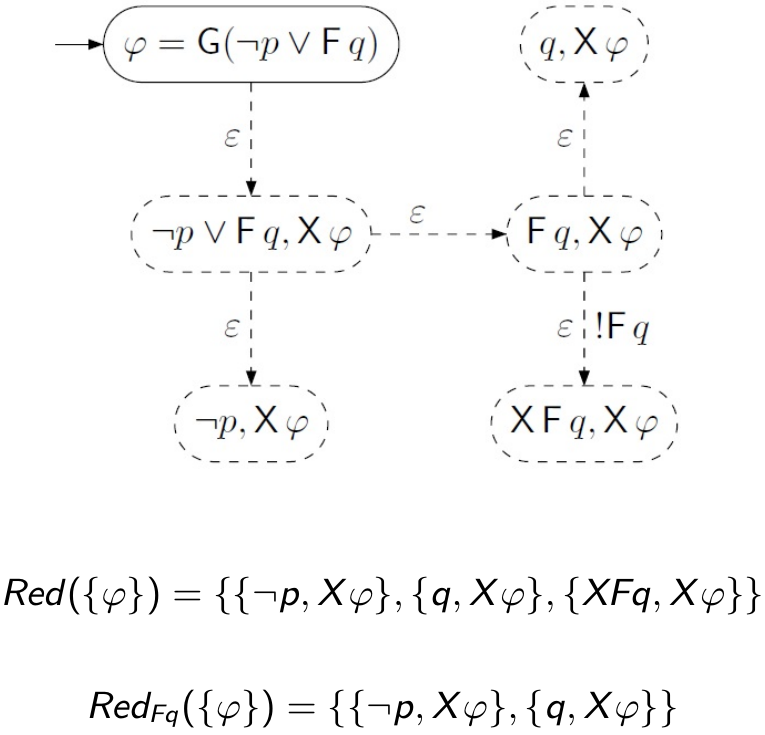
\includegraphics[scale=0.3]{ltl2gba_ex1.png}
	\caption{$\varphi = G(\neg p \lor Fq)$}
	\label{ltl2gba1}
	\end{figure}
	\begin{figure}[ht]
	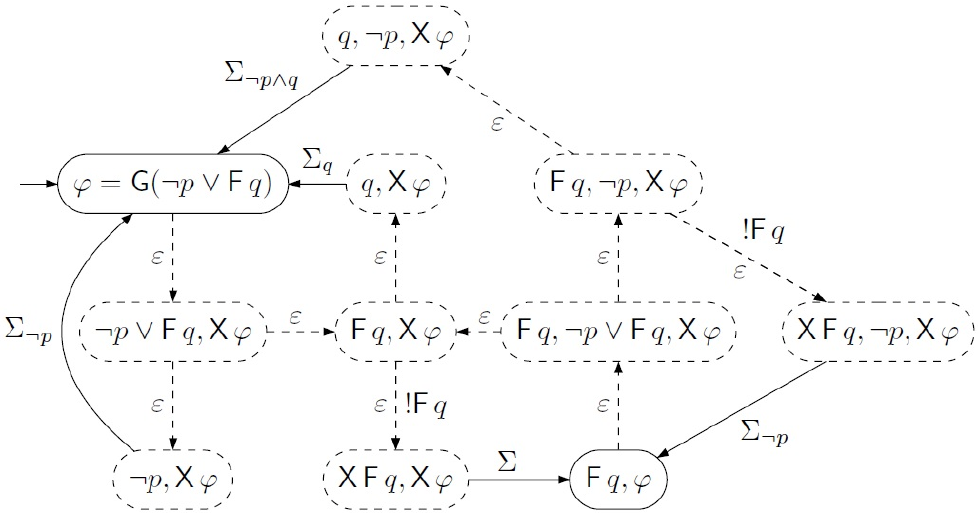
\includegraphics[scale=0.35]{ltl2gba_ex2.png}
	\caption{$\varphi = G(\neg p \lor Fq)$}
	\label{ltl2gba2}
	\end{figure}
	\begin{figure}[ht]
	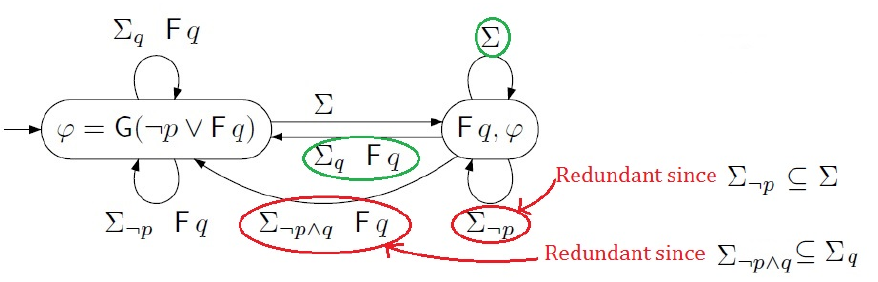
\includegraphics[scale=0.35]{ltl2gba_ex3.png}
	\caption{$\varphi = G(\neg p \lor Fq)$}
	\label{ltl2gba3}
	\end{figure}
\end{itemize}

\end{document}